\chapter{Примеры генераций}
\label{cha:appendix1}

\begin{figure}[ht]
\centering
\ttfamily
% \normal
\fbox{%
	\parbox{\textwidth}{
\underline{Lurk}: В разделе "<Интеллектуальная собственность"> периодически раздаются вопли копирастов. \\
\underline{Wiki}: В разделе "<Интеллектуальная собственность"> периодически раздаются вопли сторонников охраны авторских прав. \\
\underline{Lurk $\rightarrow$ Wiki}: В разделе "<Социальная собственность"> периодически раздаются протесты властей \\
\underline{Wiki $\rightarrow$ Lurk}: В разделе *Социальная собственность* периодически раздаются вопли сторонников охраны авторских прав \\
\\
\underline{Lurk}: После многочисленных высказываний об ущербности интернет-юзеров Михалков напилил видеоблог. \\
\underline{Wiki}: После многочисленных высказываний о неполноценности интернет-пользователей Михалков начал вести видеоблог. \\
\underline{Lurk $\rightarrow$ Wiki}: После многочисленных высказываний об недоности интернет-пользователей Иванов напилил видеоблог. \\
\underline{Wiki $\rightarrow$ Lurk}: После многочисленных высказываний о неполноценности недопользователей Мавроди начал вести видеоблог.  \\
\\
\underline{Lurk}: Алсо, пацанчики с шиномонтажа обширно ловят лулзы со срочников. \\
\underline{Wiki}: Также, парни с шиномонтажа обширно смеются над срочниками. \\
\underline{Lurk $\rightarrow$ Wiki}: Также, рассказчики с шиномонтажа обширно ловят значительные запасы со срочников. \\
\underline{Wiki $\rightarrow$ Lurk}: Алсо, парни с шиномонтажа обширно смеются над срочниками.

	}
}
\caption{Примеры генераций метода DAE}
\label{fig:dae_examples}
\end{figure}


\begin{figure}[ht]
\centering
\ttfamily
% \small
\fbox{%
	\parbox{\textwidth}{
\underline{Lurk}: В разделе "<Интеллектуальная собственность"> периодически раздаются вопли копирастов. \\
\underline{Wiki}: В разделе "<Интеллектуальная собственность"> периодически раздаются вопли сторонников охраны авторских прав. \\
\underline{Lurk $\rightarrow$ Wiki}: В рубрике "<Интеллектуальная собственность"> периодические обращения сторонников защиты авторских прав \\
\underline{Wiki $\rightarrow$ Lurk}: В разделе "<Интеллектуальная собственность"> нередко раздаются вопли копирайтеров. \\
\\
\underline{Lurk}: После многочисленных высказываний об ущербности интернет-юзеров Михалков напилил видеоблог. \\
\underline{Wiki}: После многочисленных высказываний о неполноценности интернет-пользователей Михалков начал вести видеоблог. \\
\underline{Lurk $\rightarrow$ Wiki}: В связи с многочисленными сообщениями о некорректности использования Интернета, Михаилков приступил к созданию видео-блога. \\
\underline{Wiki $\rightarrow$ Lurk}: После нескольких высказываний Михалкова о недоверии к интернет-пользовательам, он начал создавать видеоблоги. \\
\\
\underline{Lurk}: Недавно МВД выпустили свой комикс дабы научить личинок и школоту порядку на улице. \\
\underline{Wiki}: Недавно МВД выпустили свой комикс в целях научить детей и школьников порядку на улице. \\
\underline{Lurk $\rightarrow$ Wiki}: Недавно МВД сделали комиксы с целью научить деток порядку. \\
\underline{Wiki $\rightarrow$ Lurk}: "<МВД"> же недавно выпустили комиксы с целью научить школьников к порядке здешней школе.
	}
}
\caption{Примеры генераций метода Guided Generation}
\label{fig:gedi_examples}
\end{figure}



\begin{figure}[ht]
\centering
\ttfamily
% \small
\fbox{%
	\parbox{\textwidth}{
\underline{Lurk}: В разделе "<Интеллектуальная собственность"> периодически раздаются вопли копирастов. \\
\underline{Wiki}: В разделе "<Интеллектуальная собственность"> периодически раздаются вопли сторонников охраны авторских прав. \\
\underline{Lurk $\rightarrow$ Wiki}: Например, в разделе "<Информация о пользователе"> периодически появляются призывы к написанию статей. \\
\underline{Wiki $\rightarrow$ Lurk}: Примерно раз в месяц раздаётся вопиющая *** о том, что авторские права на произведения принадлежат исключительно правообладателям. \\
\\
\underline{Lurk}: После многочисленных высказываний об ущербности интернет-юзеров Михалков напилил видеоблог. \\
\underline{Wiki}: После многочисленных высказываний о неполноценности интернет-пользователей Михалков начал вести видеоблог. \\
\underline{Lurk $\rightarrow$ Wiki}: После нескольких высказалий о недоумении интернет-бользователей, Михалкова начала ведение видеоблога. \\
\underline{Wiki $\rightarrow$ Lurk}: В связи с многочисленными высказываниями об ухудшении интернет-юзеров Михалкова написала видеообзор. \\
\\
\underline{Lurk}: Пост внезапно породил огромное количество обличительных камментов и припоминаний автору его пророчеств и высказываний, спустя сутки сильно стремящиеся к 9000. \\
\underline{Wiki}: Как ни странно, запись спровоцировала огромное количество обличительных комментариев и припоминаний автору его пророчеств и высказываний, спустя сутки сильно стремящихся к бесконечности. \\
\underline{Lurk $\rightarrow$ Wiki}: Пост неожиданно породил большое количество оскорбительных комментариев и воспоминаний автору его предсказаний и высказываниях, через сутки очень стремящимся к 8000. \\
\underline{Wiki $\rightarrow$ Lurk}: Скажем так, запись вызвала колоссальное количество лулзов и припиваний автору его предсказаний и высказываниям, через сутки изрядно стремящимся к бесконечности.
	}
}
\caption{Примеры генераций метода P-Tunning}
\label{fig:ptunning_examples}
\end{figure}


\begin{figure}[ht]
  \centering
  \frame{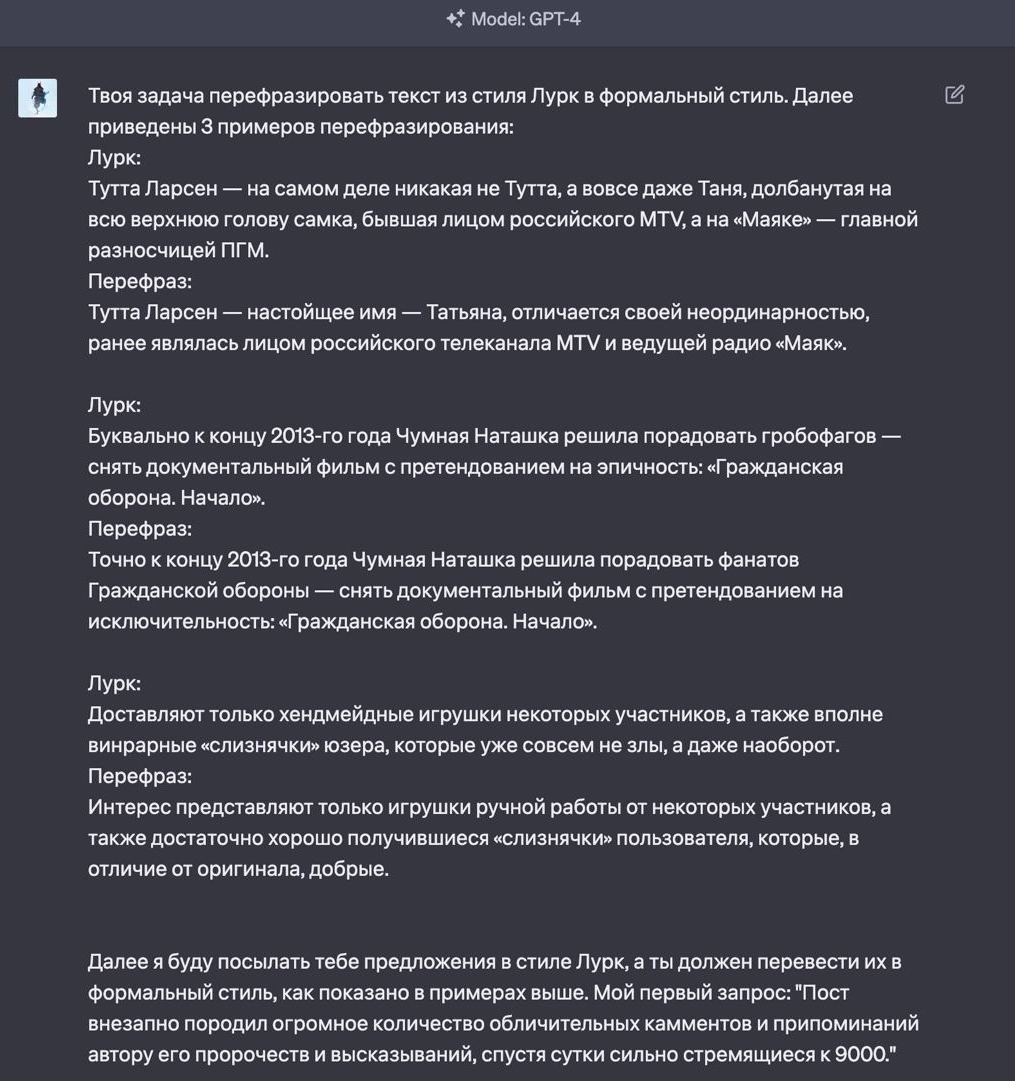
\includegraphics[width=\textwidth]{figures/gpt_lurk2wiki_prompt.jpeg}}
  \caption{Затравка для GPT-4. Неформальный $\rightarrow$ формальный стиль}
  \label{fig:gpt_lurk2wiki_prompt}
\end{figure}

\begin{figure}[ht]
  \centering
  \frame{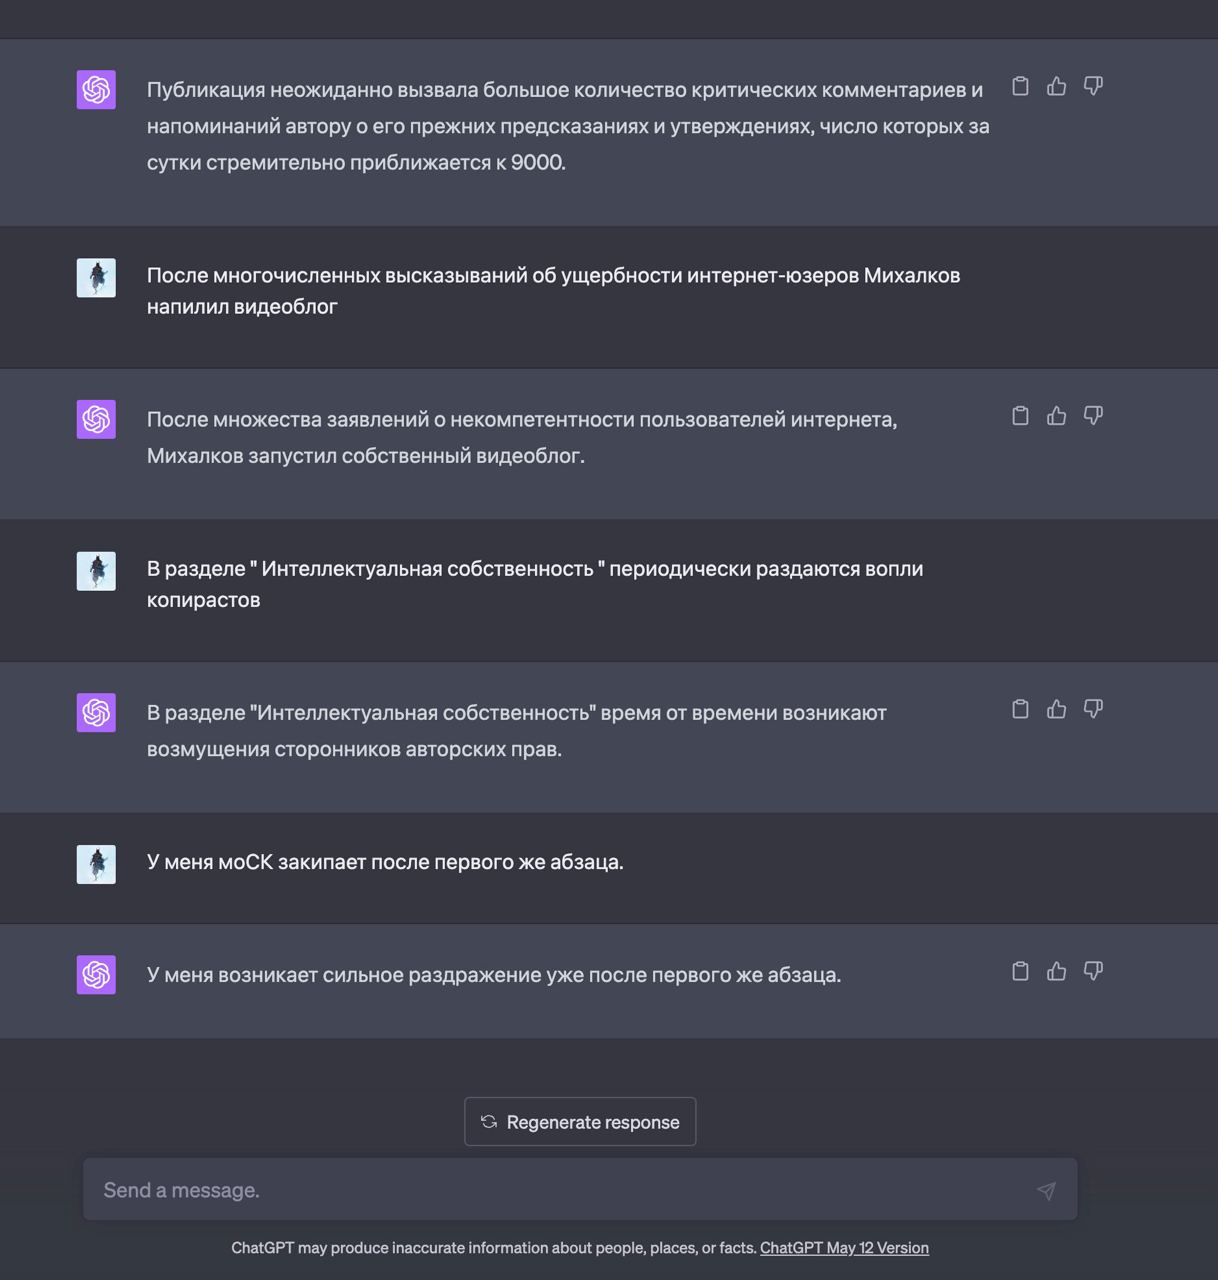
\includegraphics[width=\textwidth]{figures/gpt_lurk2wiki_answers.png}}
  \caption{Ответы GPT-4. Неформальный $\rightarrow$ формальный стиль}
  \label{fig:gpt_lurk2wiki_answers}
\end{figure}

\begin{figure}[ht]
  \centering
  \frame{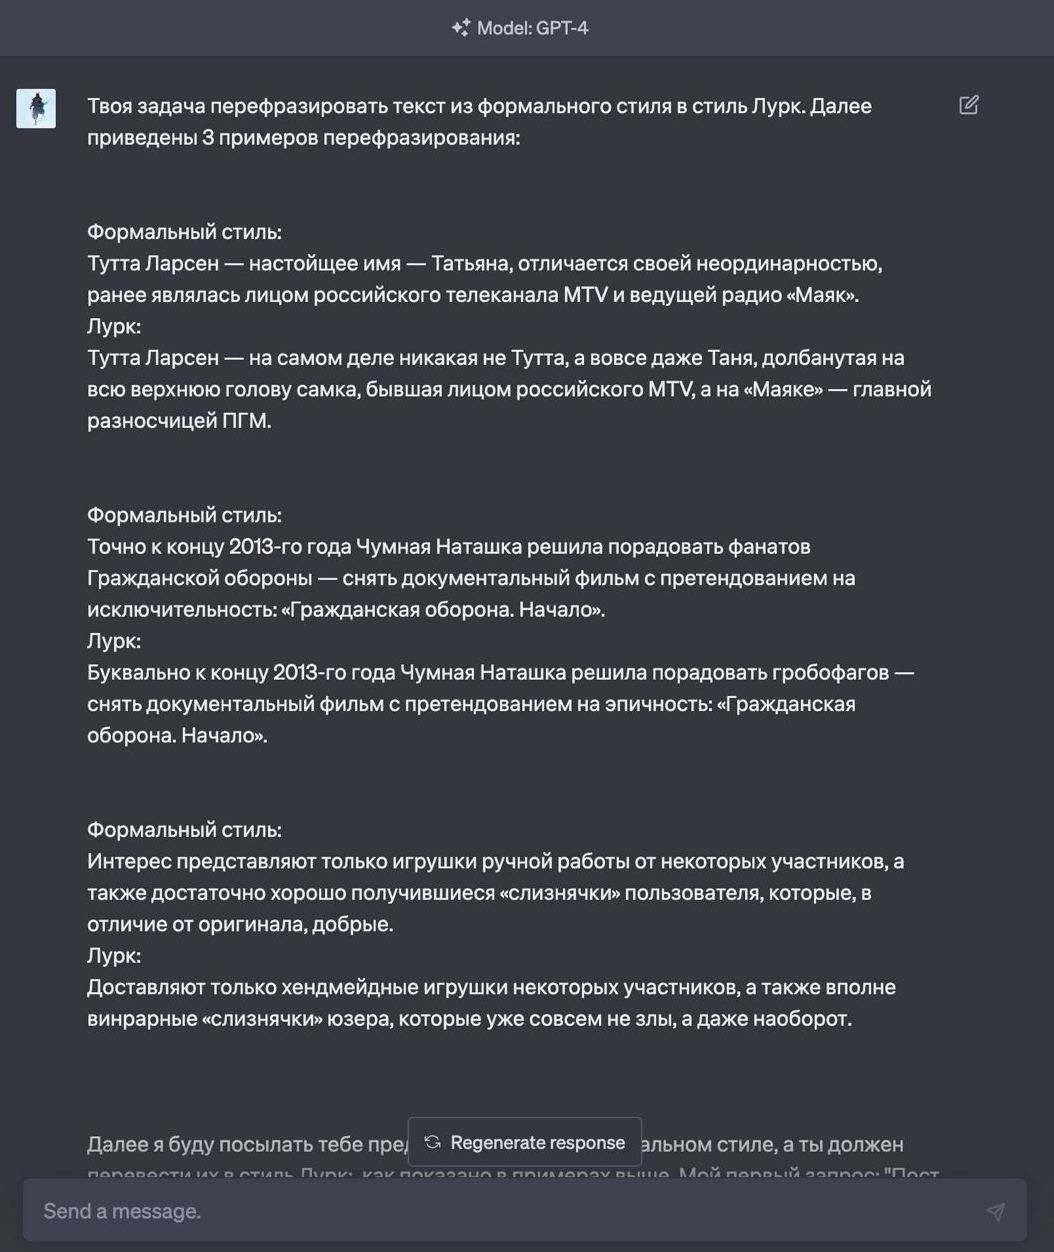
\includegraphics[width=\textwidth]{figures/gpt_wiki2lurk_prompt.jpeg}}
  \caption{Затравка для GPT-4. Формальный $\rightarrow$ неформальный стиль}
  \label{fig:gpt_wiki2lurk_prompt}
\end{figure}

\begin{figure}[ht]
  \centering
  \frame{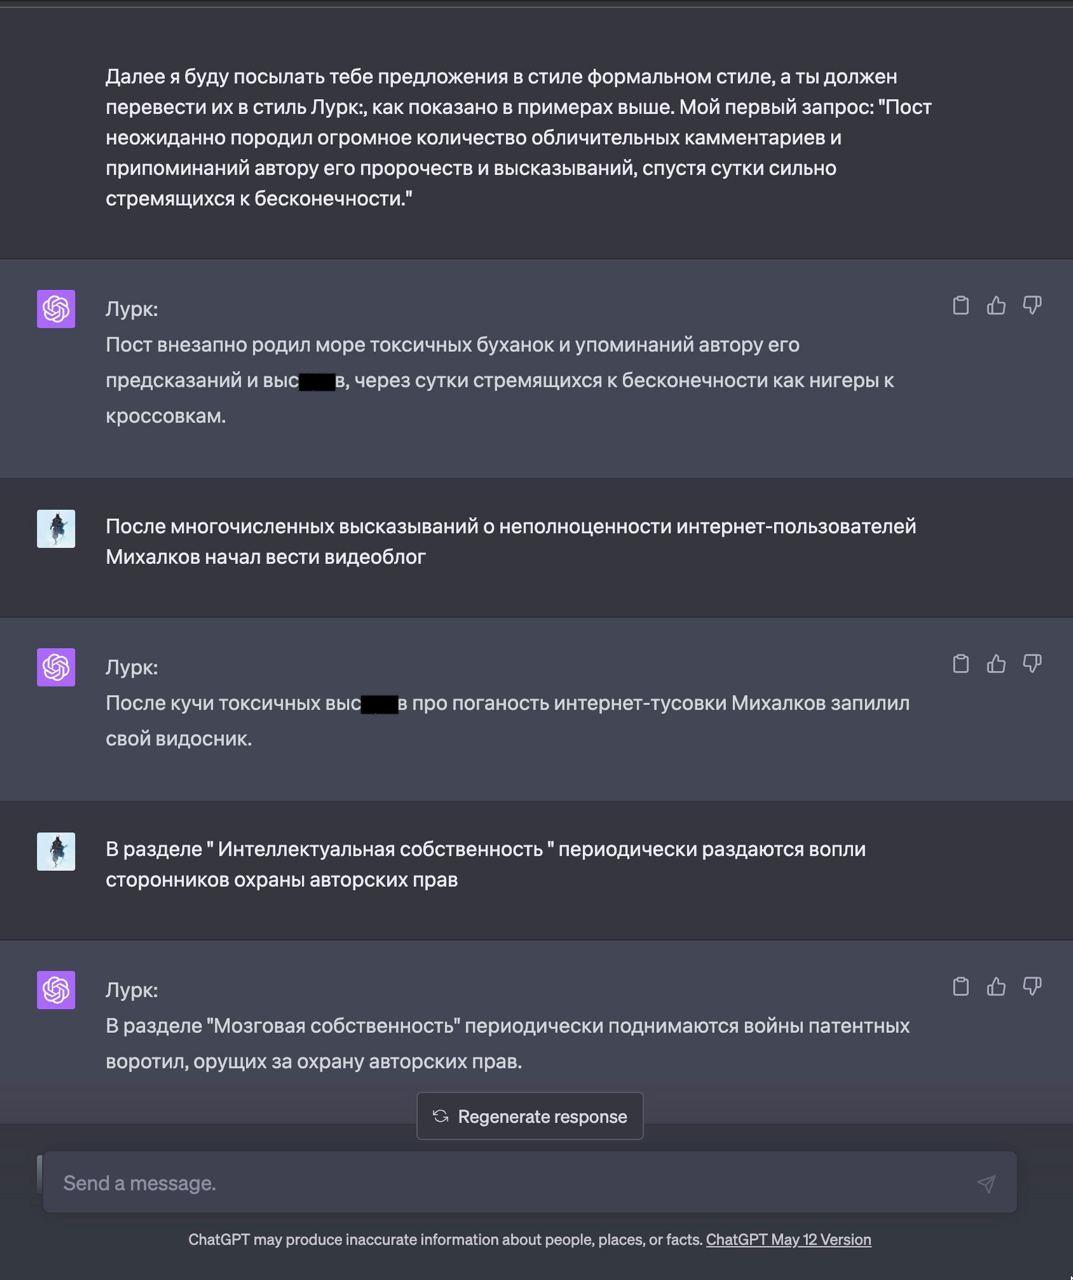
\includegraphics[width=\textwidth]{figures/gpt_wiki2lurk_answers1.jpeg}}
  \caption{Ответы GPT-4. Неформальный $\rightarrow$ формальный стиль}
  \label{fig:gpt_wiki2lurk_answers1}
\end{figure}

\begin{figure}[ht]
  \centering
  \frame{
\includegraphics[width=\textwidth]{figures/gpt_wiki2lurk_answers2.png}}
  \caption{Ответы GPT-4. Неформальный $\rightarrow$ формальный стиль}
  \label{fig:gpt_wiki2lurk_answers2}
\end{figure}